\documentclass[12pt,fleqn]{article}\usepackage{../common}
\begin{document}
Ders 20

Cizgi entegrallerini is hesabinda gormustuk. $\vec{F}$ tarafindan $C$
egrisi uzerinde yapilan isi

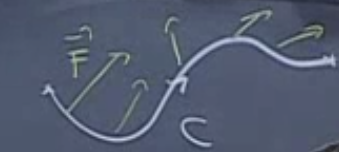
\includegraphics[height=2cm]{20_1.png}

\[ \int_C \vec{F} \cdot d\vec{r} =  \int_C \vec{F} \cdot \vec{T} ds \]

olarak gormustuk. Esitligin sagi birim teget vektoru kullanarak ayni hesabi
gosteriyor, $ds$ ise egri uzunlugu $s$'ten ortaya cikiyor. Diger bir form

\[ = \int_C M dx + N dy \]

ki $\vec{F} = <M,N>$ olmak uzere. 

Ornek 

Soyle bir vektor alani veriyorum

\[ \vec{F} = <y,x> \]

Bu alanin neye benzedigi cok bariz degil, ama bu alanin bir bilgisayar
cizimi altta

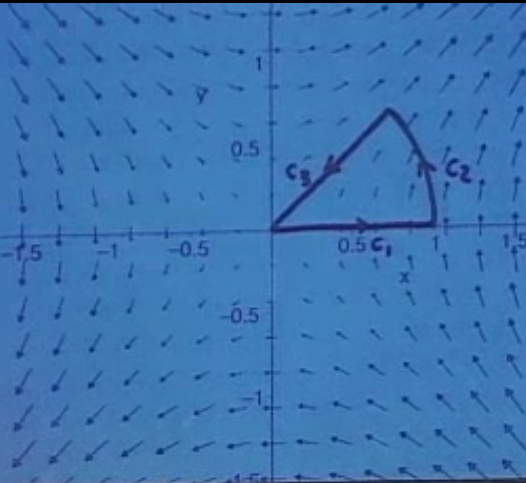
\includegraphics[height=5cm]{20_2.png}

Diyelim ki bu vektor alaninda orijinden baslayarak $c_1,c_2,c_3$
vektorlerini takip ederek hareket ettigimde yapilan isi hesaplamak
istiyorum. $c_1$ duz, $c_2$ birim cember uzerinde bir parca, $0 \le \theta
\le \pi / 4$ 
olmak uzere, ve $c_3$ tekrar duz. Yani 

\[ c = c_1 + c_2 + c_3 \]

O zaman is hesap entegralinin uc parcasi olacak. Her parca $i$ icin 

\[ \int_{C_i} y dx + x dy\]

gerekiyor. 

1) Yatay x ekseninde, $(0,0)$'dan $(1,0)$'a. 

\[ y = 0, \ dy = 0 \]

\[ \int_{c_1} y dx + x dy = 0 \ dx + 0 = 0\]

Cizgi entegrali cok basit yani. Bu sifir sonucunu baska sekilde de
gorebilirdik, vektor alanina bakarsak x eksenine her zaman dik oldugunu
gorururuz. O zaman $\vec{F}\cdot \vec{T}$ hep sifir sonucunu verecektir. 

2) $c_2$ bolumu. 

$x,y$'yi tek degisken baglaminda nasil temsil edecegimizi bulmamiz
gerekiyor. Eger bir cember uzerinde hareket ediyorsak, bu tek degisken aci
olabilir. 

\[ x = cos(\theta) \]

\[ y = sin(\theta) \]

\[ 0 \le \theta \le \pi / 4 \]

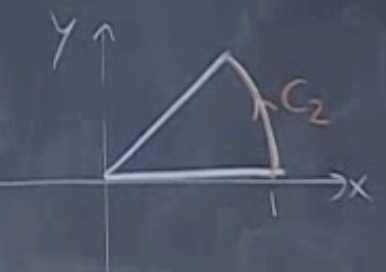
\includegraphics[height=3cm]{20_3.png}

Turevleri alirsak

\[ dx = -sin\theta \ d\theta\]

\[ dy = cos\theta \ d\theta \]

Entegral

\[ \int_{c_2} y dx + x dy = 
\int_0^{\pi/4} sin\theta (-sin\theta \ d\theta)  + 
cos\theta \ cos\theta \ d\theta
\]

\[ = \int_0^{\pi/4} cos^2\theta - sin^2\theta d\theta \]

\[ = \int_0^{\pi/4} cos(2\theta) d\theta \]

\[ = \frac{1}{2}sin2\theta \bigg|_0^{\pi/4} \]

\[ = \frac{1}{2} \]

3) $c_3$ bolumu

\[ \int_{c_2} y dx + x dy \]

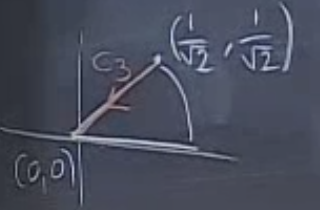
\includegraphics[height=4cm]{20_4.png}

Basladigimiz noktayi biliyoruz, geriye dogru orijine gelecegiz. Bu cizgiyi
parametrize etmek zor degil. 

\[ x = \frac{1}{\sqrt{2}} - \frac{1}{\sqrt{2}} t \]

\[ y = \frac{1}{\sqrt{2}} - \frac{1}{\sqrt{2}} t \]

\[ 0 \le t \le 1 \]

Ama ustteki dogru olsa da, gereginden fazla cetrefil oldu. 

Daha kolay bir yontem ``orijinden'' ileri dogru bir yon dusunmek, ve sonra
``bunun tersi olsun'' diyerek istedigimiz gidisati elde etmek. Yani

\[ x = t \]

\[ y = t \]

ki $t$, 0 ile $1/\sqrt{2}$ arasinda. Bu bize $(-c_3)$'u verecek, yani
$c_3$'un tersini. O zaman entegrali su sekilde gorebiliriz

\[ \int_{-c_3} = - \int_{c_3}  \]

Buradaki numara 0'dan baslamanin cebirsel temsili kolaylastirmis
olmasi. Devam edelim

\[ dx = dt \]

\[ dy = dt \]

\[ \int_{-c_3} y dx + x dy  = 
\int_{0}^{\frac{1}{\sqrt{2}}} t \ dt + t \ dt = 
\int_{0}^{\frac{1}{\sqrt{2}}} 2t \ dt = 
t^2 \bigg|_{0}^{\frac{1}{\sqrt{2}}} =
\frac{1}{2}
\]

Usttekinin tersine ihtiyacimiz olduguna gore 

\[ \int_{c_3} y dx + x dy  = -\frac{1}{2}
\]


Ya da iki ustteki entegralin sinirlarini tam ters yonde de alabilirdik,
0'dan $1/\sqrt{2}$'a gitmek yerine, $1/\sqrt{2}$'dan 0'a gidebilirdik, o da
ayni sonucu verirdi. 

Nihayet, yapilan tum is, tum entegrallerin toplami olacagina gore

\[ \int_C = \int_{c_1} + \int_{c_2} + \int_{c_3}  \]

\[ = 0 + \frac{1}{2} - \frac{1}{2} = 0\]

Peki cizgisel entegralleri hesaplamaktan kurtulabilir miyiz? 

Simdi, gordugumuzde vurgulamamis olsakDiyelim ki vektor alani $\vec{F}$ bir
fonksiyonun gradyani, yani

\[ \vec{F}  = \nabla f\]

Bir gradyan alanimiz var yani, ve bu durumda $f(x,y)$'ye bir potansiyel
alani (potential field) diyebiliriz. Bu isim fizikle alakali dogal olarak,
$f$ fonksiyonu $x,y$ noktasinda ne kadar enerji, potansiyel,
vs. depolandigini gosterir genellikle, ve bu noktadaki gradyan kuvveti
verir. Daha dogrusu gradyanin negatifi, fizikciler gradyani eksi ile
carparlar, yani matematikciler ile aralarinda boyle bir fark
vardir. Aklimizda tutalim. Biz eksi olmayan yontemi kullanacagiz.

Cizgizel Entegraller Icin Calculus'un Temel Teorisi

\[ \int_{C} \nabla f \cdot d\vec{r} = 
f(P_1) - f(P_0)
 \]

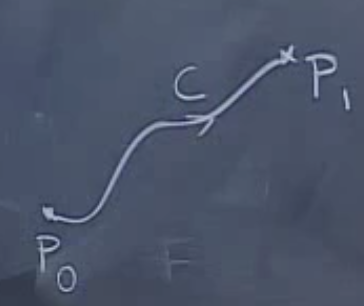
\includegraphics[height=3cm]{20_5.png}

Bu cok faydali bir formul, ama sadece vektor alani bir gradyan ise, ve
$f$'i biliyorsak ise yarar. Ileriki bir derste bir vektor alaninin bir
gradyan olup olmadigini nasil anlayacagimizi gorecegiz, ve eger bir gradyan
ise, potansiyel fonksiyonunu geri elde etmenin tekniklerini gorecegiz. 

\[ \int_C f_x dx + f_y dy  = \int_C df = f(P_1) - f(P_0) \]


Ustteki en sagdaki esitlige bakinca $f$ noktalari arasindaki fark formulunu
nasil elde ettigimiz aslinda pek sasirtici degil. Bu formda elde ettigimiz
sonuc tek degiskenli Calculus'taki sonuc ile ayni. 

Ispat

Diyelim ki size bir egri verdim ve alttaki entegrali hesaplamanizi
istedim. 

\[ \int_{C} \nabla f \cdot d\vec{r} =  \int_C f_x dx + f_y dy
 \]

Bunu nasil yapariz? Bir parametre seceriz ve her seyi o parametre
baglaminda temsil ederiz. 

\[ C: x = x(t), y = y(t) \]

O zaman 

\[ dx = x'(t)dt, dy = y'(t)dt \]

\[ \int_{C} \nabla f \cdot d\vec{r} =  
\int_C \bigg( f_x \frac{dx}{dt} + f_y \frac{dy}{dt} \bigg) dt
\]

Parantez icindeki ifadeler tanidik geliyor mu? Boyle bir sonucu Zincirleme
Kanunu sonucunda da gormustuk. 

\[ = \int_C \frac{df}{dt} dt\]

Diyelim ki $t_0 \le t \le t_1$

\[ = \int_{t_0}^{t_1} \frac{df}{dt} dt\]

Ve bildik Calculus'un Temel Teorisine gore ustteki $f$'in iki deger
arasindaki farkina esittir. 

\[ = f\bigg( x(t), y(t) \bigg) \bigg|_{t_0}^{t_1} =
f(P_1) - f(P_0)
\]

Ispat tamamlandi. 

Ornek

Bastaki ornege donersek, orada gorulen vektor alani aslinda raslantisal bir
sekilde bir gradyan alani da olabilir mi acaba? Vektor alani soyleydi

\[ \vec{F} = <y,x> \]

Acaba aklimiza $x$'e gore turevi alininca $y$, $y$'ye gore turevi alininca
$x$ olan bir fonksiyon geliyor mu? Evet, mesela $xy$ fonksiyonu boyle bir
fonksiyon. Yani

\[ f(x,y) = xy \]

O zaman bu alanda bir cizgi entegralini hesaplamak icin $f$'in baslangic,
bitis noktalari arasindaki farki almak yeterli. 

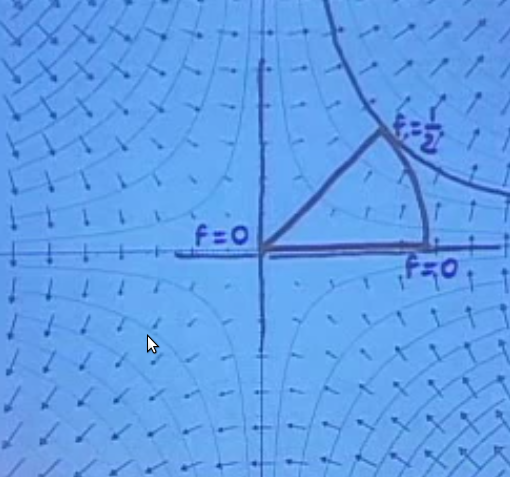
\includegraphics[height=4cm]{20_6.png}

Ustteki resmi nasil okuruz? $c_1$ boyunca potansiyel hic degismedi, yapilan
is sifir. Sonra $c_2$ boyunca hareket ve $1/2$'ye geldik, yapilan is $1/2$,
gibi. 

Bu guzel bir numara ve oldukca kullanisli, cunku cogu vektor alani bir
gradyan alani olarak gorulebiliyor, mesela fizikte potansiyelin
gradyani. Ama unutmayalim, her vektor alani gradyan degildir, gradyan
olmayan pek cok vektor alani vardir. Mesela manyetik alanlar gradyan
degildir. 

Bu uyaridan sonra, eger $\vec{F}$ bir gradyan alani ise, Temel Teorinin
diger etkilerini de gorelim. 

Sonuc 1: Yol Bagimsizligi (path independence) Ozelligi

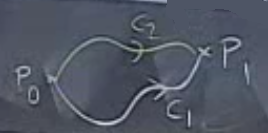
\includegraphics[height=2cm]{20_7.png}

Cizgi entegralini hesaplarken hangi yoldan gectiginiz onemli degil, eger
baslangic ve bitis noktalari ayni ise. Bu ozellik diger vektor alanlari
icin dogru olmayabilir, ama gradyan alanlari icin isler.

Resimde durum icin bu

\[ \int_{c_1}\nabla f \cdot d\vec{r} =  \int_{c_2}\nabla f \cdot d\vec{r} \]

Bu teorinin ispati aslinda kolay, Temel Teorinin yan etkilerinden biri
sadece. Baslangic ve bitis ayni ise, onlarin farki hangi yoldan gidilirse
gidilsin ayni olacaktir. 

Bu ne ise yarar? $f$'i bilmiyorsak bile eger vektor alaninin gradyan alani
oldugunu biliyorsak, cizgi entegralleri birbirine esittir diyebiliriz hemen. 

Sonuc 2: $\vec{F} = \nabla f$ Muhafazakardir (conservative)

Fizik baglaminda muhafazakarlik enerjinin muhafaza edilmesinden ileri
gelir, bu kavrama gore enerjiyi kuvvet alanimizda bedavaya elde
edemeyiz. Eger alttaki gibi ``kapali'' bir gidisat hayal edersek

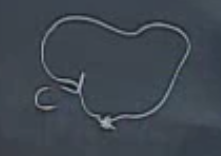
\includegraphics[height=2cm]{20_8.png}

ki $C$ bir kapali egri, o zaman $C$ uzerinde yapilan is

\[ \int_{C}\nabla f \cdot d\vec{r} = 0\]

sifira esittir. Muhafazakarligin tanimi budur. 

Fiziksel, uygulamasal olarak bunun sonucu sudur: Muhafazakar bir alanda
kapali devre, surekli kendi kendine hareket eden bir gidisat olamaz. Cunku
baslangic ve bitis arasinda yapilan is, hangi yol takip edilirse edilsin,
sifira esittir. Hic is yapilmamaktadir. 

Manyetik alanlar boyle degildir, bu sebeple bu alanlardaki hareketle o
alandan enerji cekip cikarabiliriz. Ama eletrik ve yercekimsel alanlarda bu
islemez. 

Her vektor alaninin gradyan alani olmadigini iyice vurgulamak icin su
ornege bakalim. 

\[ \vec{F} = <-y,x> \]

Bu alan bir cember etrafinda donen bir alandi. Birim cemberi (unit circle)
dusunursek $\vec{F} // \vec{T}$ idi, o zaman $\vec{F}\cdot\vec{T} =
|\vec{F}|$. Demek ki

\[ \int_C \vec{F}\cdot\vec{T} ds = \int_C \ 1 \ ds = 2\pi \]

cunku birim cember etrafinda $|\vec{F}|$ uzunlugu birim cemberin
uzunlugudur. Ve bariz bir sekilde $2\pi \ne 0$, yani bu alan muhafazakar
bir alan degil. Buradan anliyoruz ki bu alan hicbir seyin gradyani da
degil, olsaydi entegral sifir olurdu. 

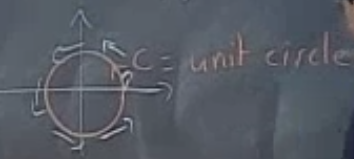
\includegraphics[height=3cm]{20_9.png}

Ek olarak yol bagimsizlik ozelligi de gecerli degil, ustteki resimde
cemberin sadece ust parcasinda hareket edersek $\pi$, alt parcasinda
hareket edersek $-\pi$ elde ederiz, bu sonuclar birbirine esit degil. 

Biraz fizik yapalim simdi.

Eger bir kuvvet alani $\vec{F}$ bir potansiyelin gradyani ise 

\[ \vec{F} = \nabla f \]

[hoca ustte eksi isareti kullanmadigi icin burada espri yaparak ``konumuz
-Fizik'' diyor]

$\vec{F}$'in yaptigi is = potansiyelin iki nokta arasindaki farki. 

Mesela yercekimsel alan, elektriksel alan ve yercekimsel potansiyel,
elektriksel potansiyel. 

Bu arada elektriksel potansiyele ``voltaj'' ismi de veriliyor, parmaginizi
prize sokunca caninizi acitan sey yani. 

[gerisi atlanti, ayni seylerden bahsediliyor]























\end{document}
